\subsection*{Problema 04}

\textbf{Enunciado:} Evaluar la integral definida 
mediante sumas de Riemann utilizando 
$\Delta x = \dfrac{5}{n}$ y 
$x_i = -2 + \dfrac{5i}{n}$:
\begin{align*}
\int_{-2}^{3} x \, dx
\end{align*}

\textbf{Solución:} 
Aplicamos la definición de la integral 
definida como el límite de una suma de 
Riemann por la derecha:
\begin{align*}
\int_{a}^{b} f(x) \, dx = \lim_{n \to \infty} 
\sum_{i=1}^{n} f(x_i) \Delta x
\end{align*}

Identificamos los datos dados:
\begin{align*}
f(x) &= x, \quad a = -2, \quad b = 3 \\
\Delta x &= \dfrac{3 - (-2)}{n} = \dfrac{5}{n}, \\
x_i &= -2 + \dfrac{5i}{n}
\end{align*}

Evaluamos la función en los puntos muestrales:
\begin{align*}
f(x_i) = -2 + \dfrac{5i}{n}
\end{align*}

Sustituimos los términos en la suma de 
Riemann:
\begin{align*}
S_n &= \sum_{i=1}^{n} f(x_i) \Delta x \\
S_n &= \sum_{i=1}^{n} \left( -2 + \dfrac{5i}{n} \right) \left( \dfrac{5}{n} \right)
\end{align*}

Expandimos y separamos la sumatoria usando 
las propiedades lineales:
\begin{align*}
S_n &= \dfrac{5}{n} \sum_{i=1}^{n} (-2) 
+ \dfrac{25}{n^2} \sum_{i=1}^{n} i \\
S_n &= \left( -\dfrac{10}{n} \right) \sum_{i=1}^{n} 1 
+ \dfrac{25}{n^2} \sum_{i=1}^{n} i
\end{align*}

Aplicamos las fórmulas de suma notables:
\begin{align*}
\sum_{i=1}^{n} 1 = n, \quad 
\sum_{i=1}^{n} i = \dfrac{n(n+1)}{2}
\end{align*}

Sustituimos estos resultados en $S_n$:
\begin{align*}
S_n &= \left( -\dfrac{10}{n} \right) (n) 
+ \dfrac{25}{n^2} \left[ \dfrac{n(n+1)}{2} \right] \\
S_n &= -10 + \dfrac{25(n^2 + n)}{2n^2} \\
S_n &= -10 + \dfrac{25}{2} \left( 1 + \dfrac{1}{n} \right)
\end{align*}

Calculamos el límite cuando $n \to \infty$ 
para obtener el valor exacto de la integral:
\begin{align*}
\int_{-2}^{3} x \, dx &= \lim_{n \to \infty} S_n \\
&= \lim_{n \to \infty} \left[ -10 + \dfrac{25}{2} \left( 1 + \dfrac{1}{n} \right) \right] \\
&= -10 + \dfrac{25}{2} (1 + 0) \\
&= -10 + 12.5 = 2.5 = \dfrac{5}{2}
\end{align*}

El valor de la integral definida es $\dfrac{5}{2}$.

\begin{figure}[H]
	\centering
	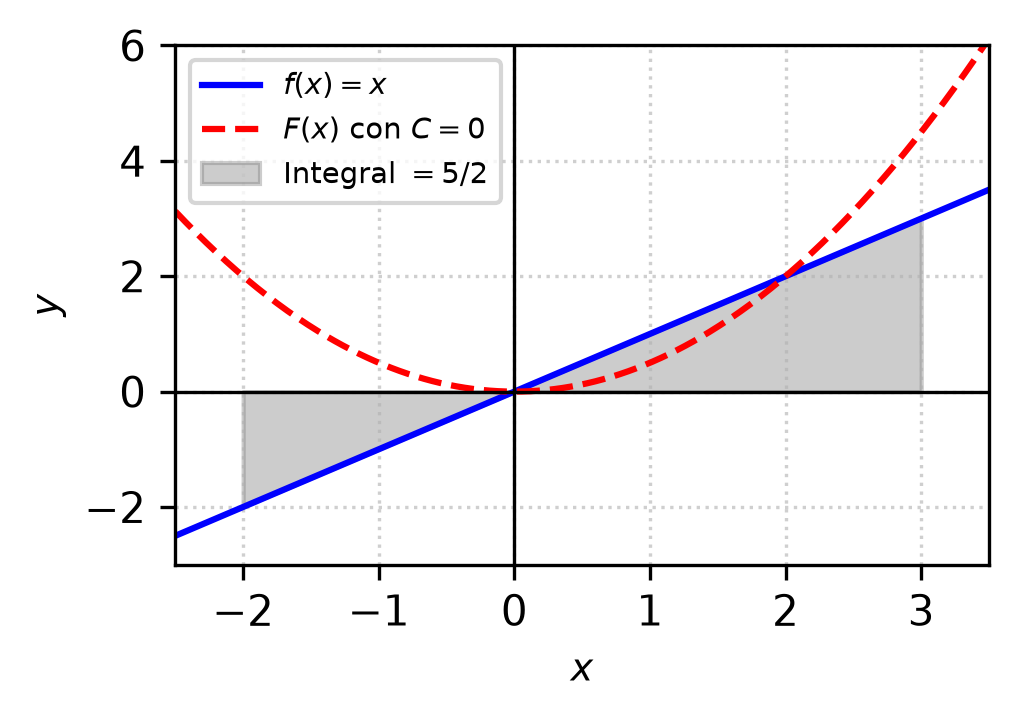
\includegraphics[width=\columnwidth]{semana_06/graficas/SEM06_P04_grafica.png}
	\caption{Representación gráfica de $f(x)$ y su antiderivada $F(x)$ evaluada para la constante de integración $C = 0$ (Problema 04).}
	\label{fig:problema04}
\end{figure}
